% Figure 1.4 (Session 1): superexchange on the half-filled Hubbard dimer.
% The image is rendered by figures/blender/s1_4_superexchange.py; the coordinates of the labels
% come from figures/blender/out/superexchange_anchors.tex. Compile with:
%   pdflatex superexchange.tex ; result moves to ../classical_magnetism/superexchange.pdf
\documentclass[11pt,tikz,border=0pt]{standalone}
\usepackage{amsmath,amssymb,graphicx}
\usepackage{xcolor}
\definecolor{coursedark}{HTML}{1B2A4A}
\definecolor{costamber}{HTML}{B8620A}
\newlength{\figw}\setlength{\figw}{16.19cm}   % the text width of the notes (letter, 2.7 cm margins), so labels print at size

\begin{document}
\begin{tikzpicture}[lbl/.style={font=\small, text=coursedark}]
  \node[anchor=south west, inner sep=0pt] at (0,0)
    {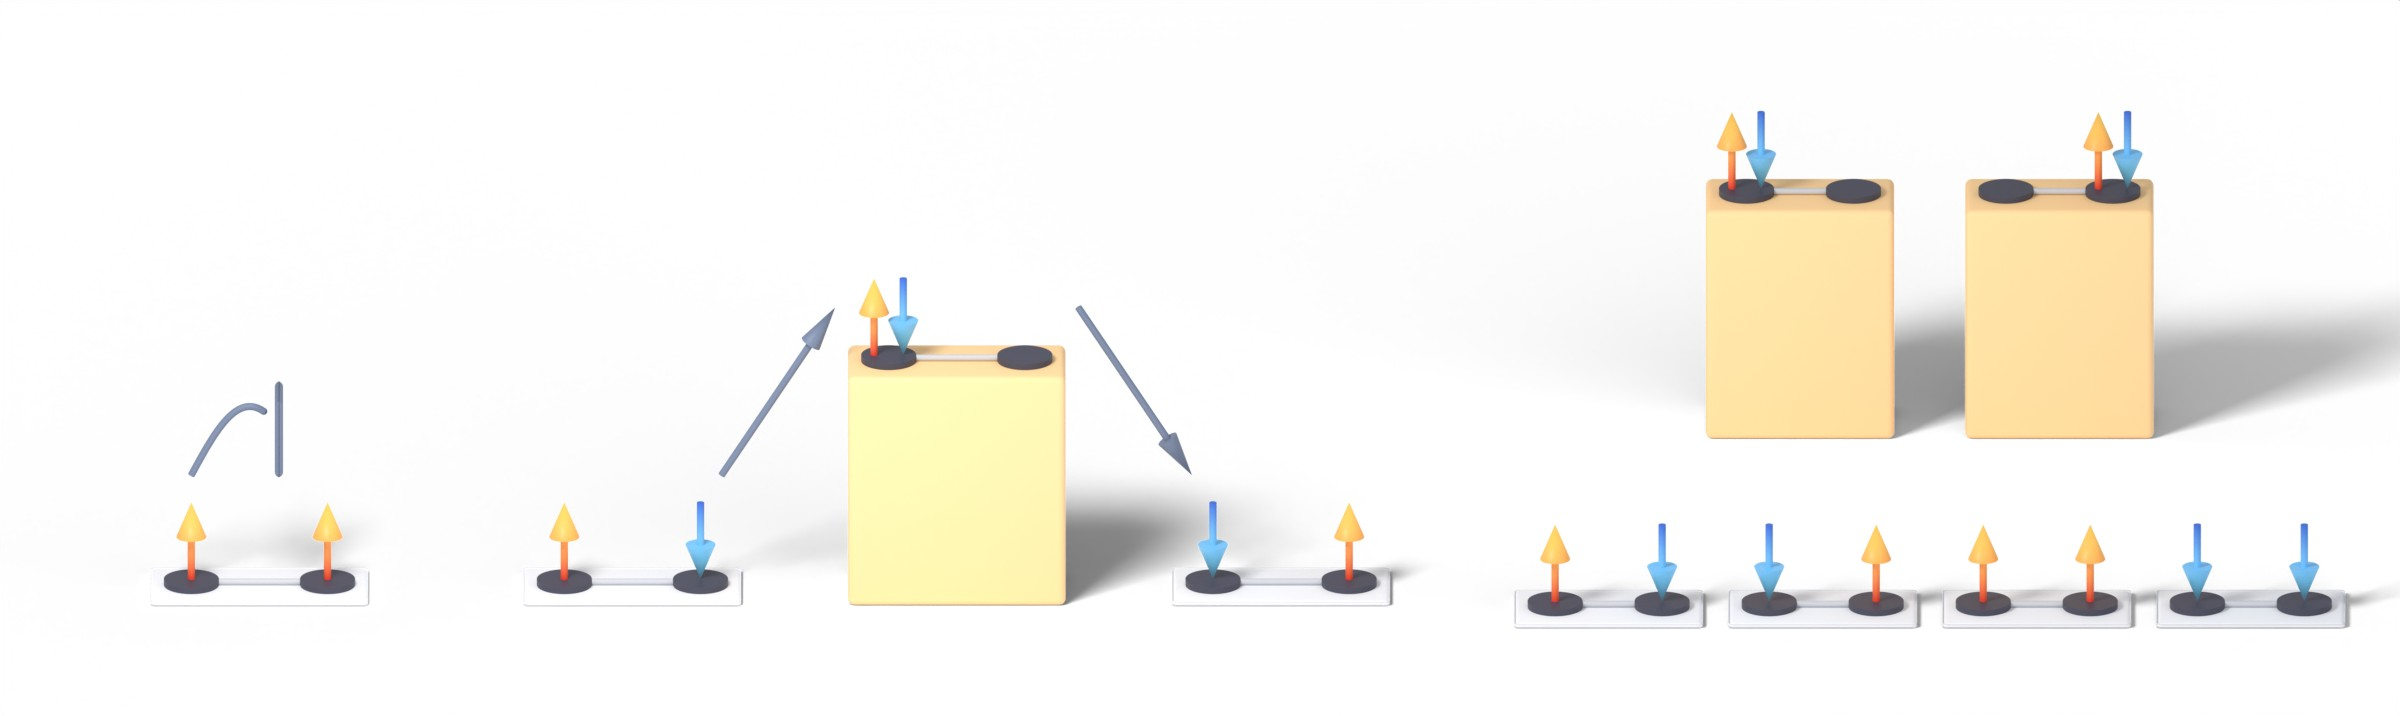
\includegraphics[width=\figw]{../blender/out/superexchange.jpg}};
  %% written by figlib.py; x and y in units of the image width
\coordinate (pauli) at (0.1250\figw,0.1353\figw);
\coordinate (E0a) at (0.1081\figw,0.0435\figw);
\coordinate (a) at (0.0270\figw,0.1893\figw);
\coordinate (t1) at (0.3209\figw,0.1480\figw);
\coordinate (t2) at (0.4764\figw,0.1480\figw);
\coordinate (Ub) at (0.4459\figw,0.1004\figw);
\coordinate (E0l) at (0.2635\figw,0.0435\figw);
\coordinate (E0r) at (0.5338\figw,0.0435\figw);
\coordinate (b) at (0.1959\figw,0.1893\figw);
\coordinate (E0c) at (0.8041\figw,0.0343\figw);
\coordinate (Uc) at (0.8953\figw,0.1888\figw);
\coordinate (c) at (0.6115\figw,0.1893\figw);

  \node[lbl, font=\normalsize, anchor=west] at (a) {(a)};
  \node[lbl, font=\normalsize, anchor=west] at (b) {(b)};
  \node[lbl, font=\normalsize, anchor=west] at (c) {(c)};
  \node[lbl, anchor=west] at (pauli) {Pauli};
  \node[lbl, anchor=north] at (E0a) {$E=0$};
  \node[lbl, anchor=south east] at (t1) {$-t$};
  \node[lbl, anchor=south west] at (t2) {$-t$};
  \node[lbl, text=costamber, anchor=west] at (Ub) {$U$};
  \node[lbl, anchor=north] at (E0l) {$E=0$};
  \node[lbl, anchor=north] at (E0r) {$E=0$};
  \node[lbl, anchor=north] at (E0c) {four states at $E=0$};
  \node[lbl, text=costamber, anchor=west] at (Uc) {two at $U$};
\end{tikzpicture}
\end{document}
